Per the experimentation workflow in Figure \ref{fig:fig12}, the final step is to save the model's parameters (state) to a \path{.pth} file. Within this file is the full ``raw" state of the learned GPyTorch model parameters. Saving this to a file allows one to simply load the model's state back into an ExactGP module and perform inference without the need for any further training. To prepare the GPyTorch model for a prototype deployment in CLEMAP's environment and infrastructure, the focus will be on developing a Docker container for the \textit{inference} phase which consists only of the ExactGP module, model state, and kernel and data utilities. In the sections below, aspects of machine learning deployment, in particular model preparation and Docker containers, as well as how a Docker container is developed is presented.

\subsection{Docker for Machine Learning Deployment}

In order to maximize business value, the deployment of new systems into a production environment must be done smoothly and at low risk. \ac{CI/CD} pipelines are a set of modern software engineering best practices to achieve the goal of releasing applications more often and faster, while also better controlling quality, risk, and costs \cite{dreyfus-schmidt_introducing_2020}. CI/CD also applies to machine learning deployment workflows and is a critical part of the ``DevOps" side of machine learning, also known as ``MLOps". An example of a ``MLOps" deployment process could contain the following steps:

\begin{figure}[H]
\centering
\graphicspath{ {./images/} }
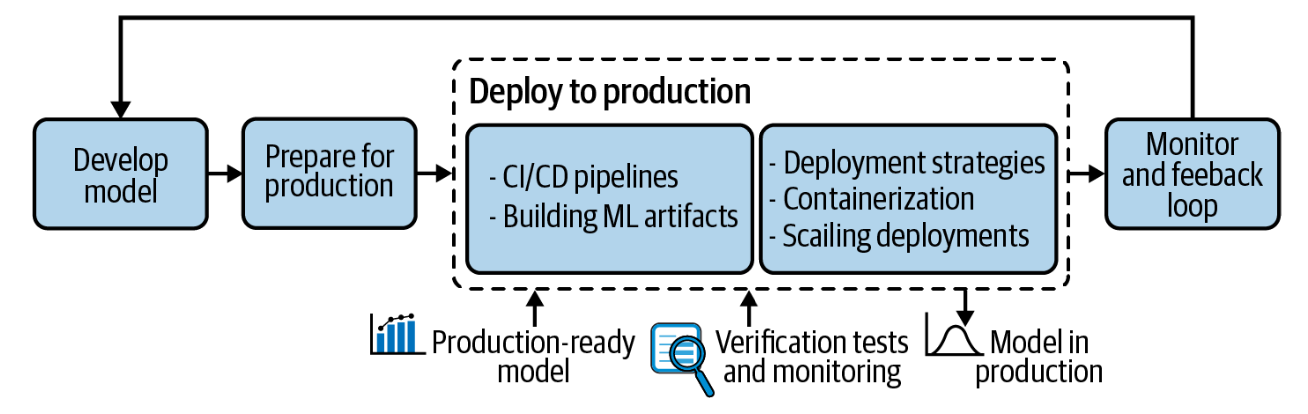
\includegraphics[scale=0.49]{images/ml_workflow.png}
\caption{Hypothetical ``MLOps" deployment process. Figure taken from \cite{dreyfus-schmidt_introducing_2020}.}
\label{fig:fig18}
\end{figure}

With the energy baseline models now developed, the focus will be on the \textit{prepare for production} phase. To prepare a model for deployment means to manage the version of a model such that an exact description of the environment (including, for example, all the Python libraries used as well as their versions, the system dependencies that need to be installed, etc.). In addition to this metadata, deployment of a model to production should automatically and reliably rebuild the environment the environment on the target machine \cite{dreyfus-schmidt_introducing_2020}. 

To achieve these goals, containerization technology is used. This technology bundles the application together with all of its related configuration files, libraries, and dependencies that are required to run across different environments \cite{dreyfus-schmidt_introducing_2020}. The specific software used for containerization in this thesis is Docker. Docker \footnote[3]{https://www.docker.com/} is an open source platform that offers container technologies, lightweight alternatives to a \ac{VM}, allowing applications to be deployed in independent, self-contained environments, matching the exact requirements of the environment that the model was developed on \cite{dreyfus-schmidt_introducing_2020}. Containerization of models is becoming a popular solution to the difficulties of dependencies when deploying machine learning models. 

Additionally, there are two ways to approach model deployment in the \textit{deploy to production} phase of Figure \ref{fig:fig18}. Namely,

\begin{itemize}
    \item Batch learning: The whole data set is available before training starts. For example, daily or weekly scheduled jobs / re-training of models.
    \item Online learning: The data set arrives sequentially in an unbounded stream. For example, a model predicts and recursively updates for each data point.
\end{itemize}

The models in this thesis were developed using the batch learning architecture as the entire data set was available before training. Although there are two ways to approach model deployment, the problem of model versioning, dependencies, and meta data still persists. Therefore, containerization technology is still utilized for both batch and online learning. 

Putting the inference phase into a container also allows for the orchestration of other containers in CLEMAP's environment. For example, their \ac{ETL} process is in a container, and by also having an inference container, these two can be orchestrated together such that the inference container is orchestrated (``runs") with the ETL container. 

\subsection{Developing a Docker Container}

There are three main components, which are developed successively, to build a Docker container:

\begin{enumerate}
    \item Dockerfile: a blueprint for building images.
    \item Docker image: a template for running containers.
    \item Docker container: the container itself, which is the packaged piece of software / application.
\end{enumerate}

In the Dockerfile, is a set of commands such as installation of python requirements from the \path{requirements.txt} file and which file to run. In the main branch of the GitHub repository, this is the \path{__main__.py} file in the \path{src} directory. After defining the Dockerfile, a Docker image, a lightweight standalone executable package of software that includes everything needed to run the application, is built. Upon successful building of the Docker image, the container can be ran, which will run the \path{__main__.py} file. Subsequently, there is the possibility of pushing the Docker container to Docker Hub, a platform similar to GitHub where repositories can be created to manage containers, to be available for use by the CLEMAP team. However, in practice, many organizations do not do this due to privacy and security concerns.